\chapter{Methods}
\label{sec:methods}

\section{Data}
\label{sec:data}

The majority of the explanatory variables used in this study are derived from the fiscal reports made available by the National Treasury Secretariat (NTS), who is responsible for collecting primary fiscal data from subnational governments in Brazil. The consolidated dataset is available at \url{https://github.com/fjuniorr/junior2017}. The focus of this section is to present an exploratory and descriptive analysis of the fiscal indicators that are used (or whose use is proposed in the new methodology) by the NTS in its payment capacity evaluation.

The final dataset used in this study consists of fiscal indicators compiled for the 26 states and the federal district from 2008 through 2016, totaling $n = 243$ observations. Since the explanatory variables will be lagged 1 year, the sample size is reduced from 2009-2016, totaling $n = 216$ for estimation purposes.

For the purposes of this study, the publication of a decree of financial calamity\footnote{\url{http://economia.estadao.com.br/noticias/geral,veja-por-que-os-estados-decretam-calamidade-financeira,10000096967}} will be the event that characterizes a fiscal crisis in a given state-year. The reasoning is that, consistent with the discussion made in section \ref{sec:fiscal-distress}, the decree of public calamity, although legally questionable\footnote{\url{http://g1.globo.com/bom-dia-brasil/noticia/2016/12/calamidade-financeira-de-estados-nao-e-reconhecida-pelo-governo.html}}, clearly signals that the policy mix has become unsustainable, and, even if there are still doubts about the states ability to pay in terms of solvency and liquidity, definitely they don't have the willingness to pay. Therefore the dummy default $d_{it}$ will take the value of one in 2016 for the states of Rio de Janeiro (RJ), Rio Grande do Sul (RS), and Minas Gerais (MG). Following previous studies, we will use the time-horizon of one year $h=1$, meaning that the forward-looking independent variable $y_{it}$ will be equal to $d_{it}$. 

Table \ref{tbl:desc_stats} presents descriptive statistics for the explanatory variables that will be used in this study. With respect to the fiscal indicators of the current methodology, four variables are especially different in the non-calamity/calamity dichotomy.  These variables show that the states that did not declared financial calamity have lower debt (Gross debt / Net current revenue - $0.86 \pm 0.56$ \textit{vs} $2.19 \pm 0.13$), a less expensive payroll cost (Compensation of employees / Net current revenue - $0.54 \pm 0.09$ \textit{vs} $0.74 \pm 0.04$), more savings (Current fiscal balance / Current revenue - $0.23 \pm 0.17$ \textit{vs} $0.00 \pm 0.12$) and more investments (Gross investment in nonfinancial assets / Total expenditure - $0.09 \pm 0.04$ \textit{vs} $0.03 \pm 0.01$) than those states that did declare financial calamity. The ratio Primary balance / Debt Service also shows that the calamity states were running on average a primary deficit ($-0.66 \pm 1.00$), although with too much variability overall to characterize the differences between the two groups. The same holds true for the ratio Social contributions / Social benefits that shows that the states that declared calamity on average have a larger social security deficit, although with large variability overall.

In regard to the fiscal indicators proposed by the new methodology, the non-calamity/calamity difference is startling. Besides the already identified higher debt and lower savings of calamity states, they have very large liquidity problems compared to the non-calamity states (Current liabilities / Cash and cash equivalents - $0.47 \pm 0.36$ \textit{vs} $2.57 \pm 0.70$). Although with the data available it is not possible to distinguish how big is the arrears stock, this proxy indicates that the number is likely to be very large for calamity states.

\begin{table}[!ht]
\centering
\caption{Descriptive statistics} \label{tbl:desc_stats}
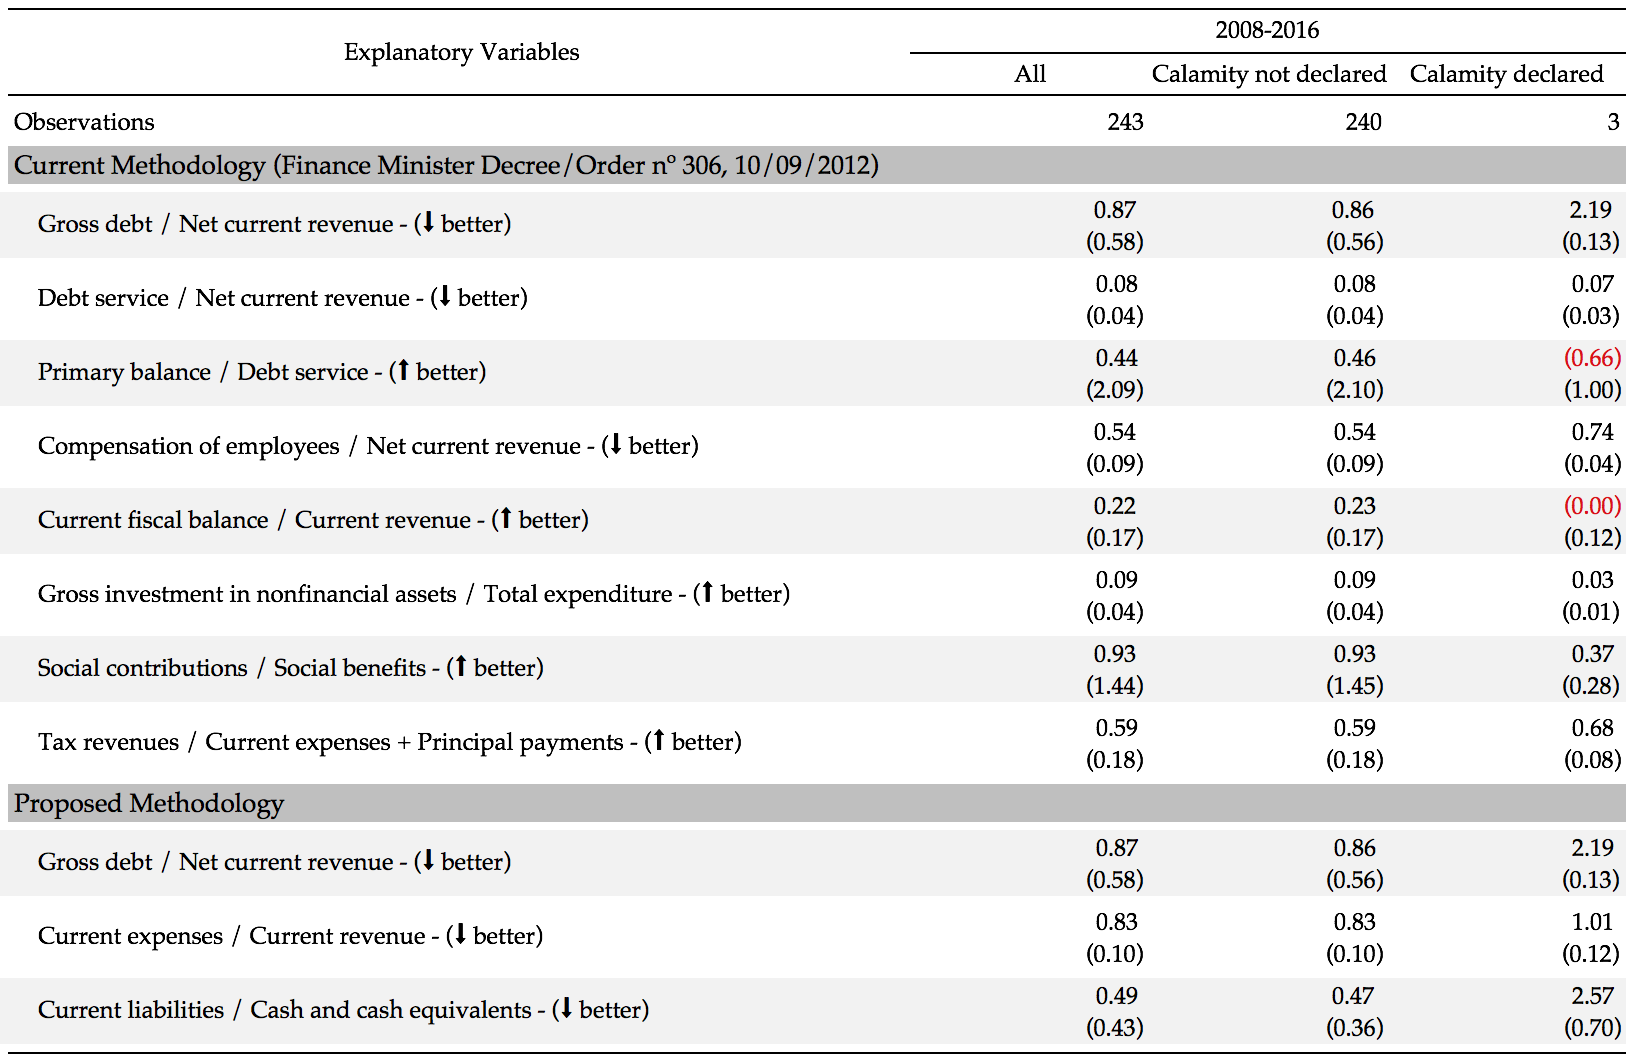
\includegraphics[scale=0.50]{tables/desc_stats.png}
\fnote{Notes: \\
       1) All variables are reported as averages across the observations with standard deviation reported in parentheses \\
       2) The variable Gross debt / Net current revenue is reported twice only to acknowledge that it was present in both methodologies. The variables Current fiscal balance / Current revenue and Current expenses / Current revenue have a different calculation rule, but convey the same information. For econometric purposes, only one will be used to avoid multicollinearity issues}
\end{table}

One particular feature of the data that is not possible to gauge from table \ref{tbl:desc_stats} is for how long the states that declared financial calamity in 2016 had worse fiscal indicators than the other states. Figure \ref{fig:evolution_capag} shows this evolution for the fiscal indicators of the new methodology. The major trend is that in the whole 2008-2016 the two groups of states were different, but, the states that declared financial calamity in 2016 had a major fiscal deterioration in 2015 and 2016. The evolution of Current liabilities / Cash and cash equivalents is particularly marked, going from an average of $0.98$ in 2014, to $1.88$ in 2015 and ballooning to $2.57$ in 2016.

\begin{figure}[!ht]
\centering
\begin{subfigure}{.5\textwidth}
  \centering
  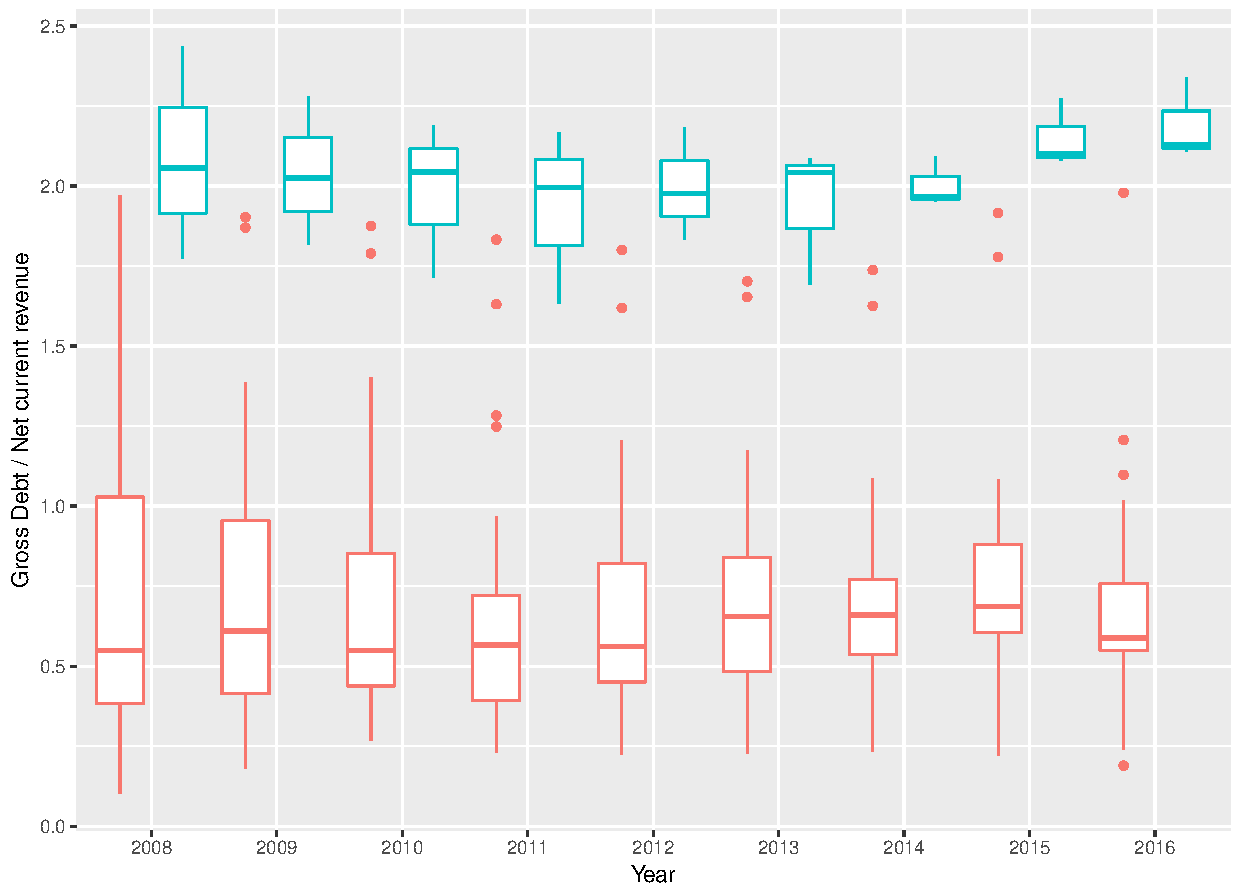
\includegraphics[width=\linewidth]{viz_capag_idc.pdf}
  \caption{Gross Debt / Net current revenue}
  \label{fig:capag_pc}
\end{subfigure}%
\begin{subfigure}{.5\textwidth}
  \centering
  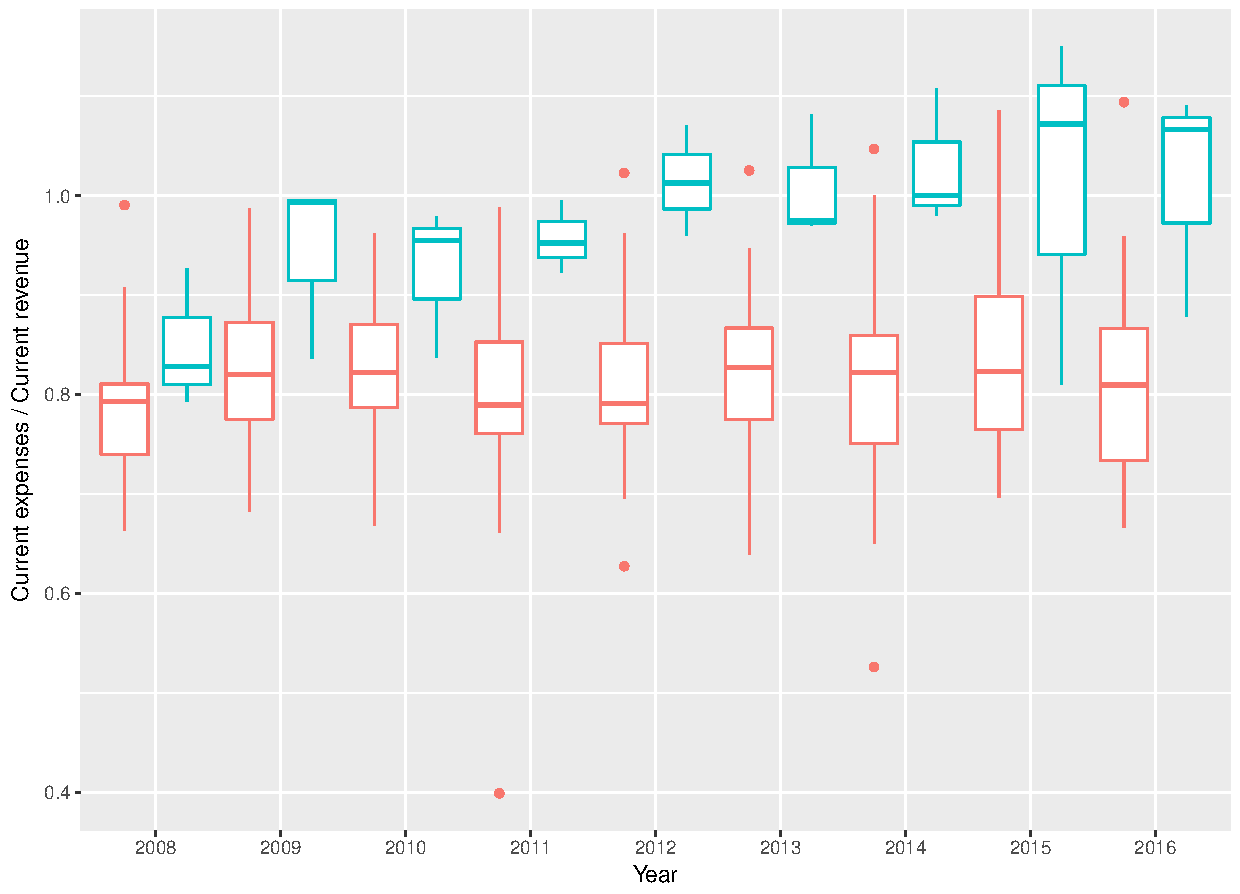
\includegraphics[width=\linewidth]{viz_capag_pc.pdf}
  \caption{Current expenses / Current revenue}
  \label{fig:capag_il}
\end{subfigure}

\begin{subfigure}{\textwidth}
  \centering
  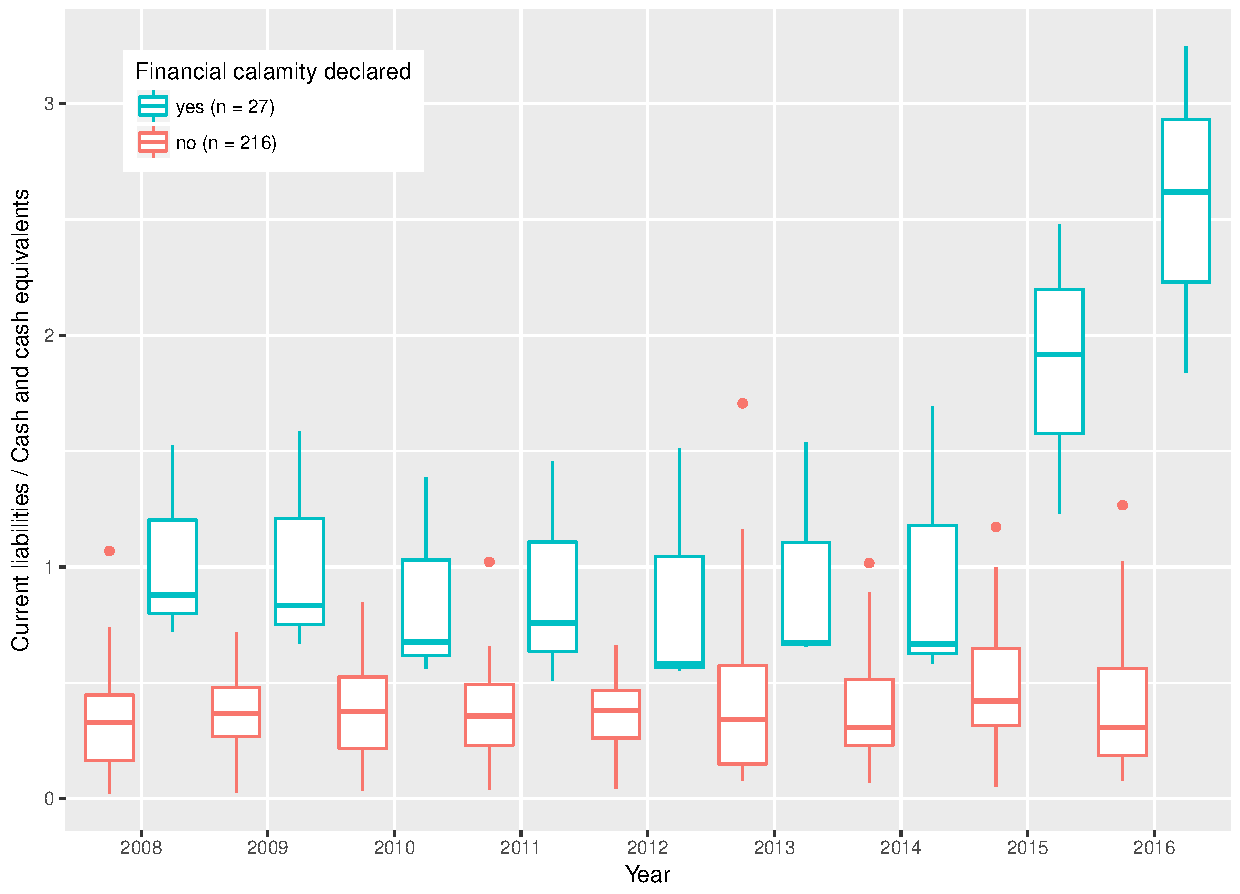
\includegraphics[width=\linewidth]{viz_capag_il.pdf}
  \caption{Current liabilities / Cash and cash equivalents}
  \label{fig:capag_idc}
\end{subfigure}%

\caption{Evolution of SGNs Financial Ratios proposed in the Payment Capacity Evaluation - 2008-2016}
\label{fig:evolution_capag}
\caption*{Source: Own elaboration}
\end{figure}

\clearpage

\section{Econometric Model}
\label{sec:econometric-model}

In this section we mostly follow the expositions and results from \citet{greene2011}, \citet{heij2004} and \citet{davidson2004} adapted to the notation used in this study. 

To assess the relative importance of these several potential explanatory variables, we need to use multiple regression analysis. The main model in this study will be a logit model, which is a special case of a binary response model. The binary response model can be derived from an underlying latent variable model. The latent variable model is
\begin{equation}
y^*_{it} = \vx'_{i,t-1}\vbeta + \epsilon_{it}, \quad (i = 1, \dots, N \text{ and } t = 1, \dots, T)
\end{equation}

This is the so-called index function, $\vx_{i,t-1}'\vbeta$ is the systematic term and $\epsilon_{it}$ is an idiosyncratic error term. In our case, the latent variable $y^*_{it}$ can be interpreted as either a propensity to default or as a measure of creditworthiness. We don't observe $y^*_{it}$, only $y_{it}$ according to
\begin{equation}
y_{it} = \begin{cases} 
      1, & \text{if } y^*_{it} \geq 0 \\
      0, & \text{if } y^*_{it} < 0 
   \end{cases}
\end{equation}
Assuming that $\epsilon_{it}$ has a standard logistic distribution we have that
\begin{align}
\label{eq:model}
\begin{split}
\Pr(y_{it} = 1 \mid \vx_{i,t-1}) &= \Pr(y^*_i \geq 0 \mid \vx_{i,t-1}) \\
&= \Pr(\vx_{i,t-1}'\vbeta + \epsilon_{it} \geq 0 \mid \vx_{i,t-1}) \\
&= \Pr(\epsilon_{it} \geq - \vx_{i,t-1}'\vbeta \mid \vx_{i,t-1}) \\
&= 1 - \Lambda(-\vx_{i,t-1}'\vbeta) \\
&= \Lambda(\vx_{i,t-1}' \vbeta) \\
% &= \frac{e^{\vx_{i,t-1}' \vbeta}}{1 + e^{\vx_{i,t-1}' \vbeta}}
\end{split}
\end{align}

The density (pmf) for each observation is given by
\begin{equation*}
f(y_{it} \mid \vx_{i,t-1}) = \Lambda(\vx_{i,t-1}' \vbeta)^{y_{it}} + [1 - \Lambda(\vx_{i,t-1}' \vbeta)]^{1 - y_{it}}
\end{equation*}


Therefore the log-likelihood $\ell(\vbeta)$ for a random sample of size $n = N \cdot T$ is given by
\begin{align}
\label{eq:log-likelihood}
\begin{split}
\ell(\vbeta) &= \ln{\left(\prod_{i=1}^N \prod_{t=1}^T{f(y_{it} \mid \vx_{i,t-1})}\right)} = \sum_{i=1}^N\sum_{t=1}^T{\ln{f(y_{it} \mid \vx_{i,t-1})}} \\[5pt]
&= \sum_{i=1}^N\sum_{t=1}^T{y_{it} \cdot \ln [\Lambda(\vx_{i,t-1}' \vbeta)] + (1 - y_{it}) \cdot \ln [1 - \Lambda(\vx_{i,t-1}' \vbeta)]}
\end{split}
\end{align}

Maximization of \ref{eq:log-likelihood} with respect to $\vbeta$ gives the maximum likelihood estimates. 

\subsubsection{Perfect Classifier}

A common problem in applied work with binary dependent variables occurs whenever there is a linear combination of the explanatory variables that can perfect classify every observation. That is
\begin{equation}
y_{it} = \begin{cases} 
      1, & \text{when } \vx'_{i,t-1}\vbeta > 0 \\
      0, & \text{when } \vx'_{i,t-1}\vbeta < 0 
   \end{cases}
\end{equation}

This phenomenon is called complete separation, and it produces infinite parameter estimates in the usual numerical optimization algorithms that attempt to make the value of \ref{eq:log-likelihood} as close to zero as possible. \citet{davidson2004} gives three main reasons for the occurrence of this phenomenon in practice. The sample size is very small, the model fits extremely well, or the dataset is characterized by a much larger proportion of $1s$ or $0s$. It is likely the case that this study fulfills all three criteria, and therefore a different estimation procedure is warranted. We make use of a maximum penalized likelihood estimation first suggested by \citet{firth1993} and implemented by \citet{brglm} in the R-package \texttt{brglm}. The advantage of this procedure is that the even in cases of complete or quasi-complete separation the estimates and their standard errors are always finite \citep{brglm}.

\subsubsection{Inference and Goodness of fit}

Inference on the logit model can be conducted in the usual fashion. The significance of individual explanatory variables can be tested by the usual t-test and the significance of joint variables can be tested by the likelihood ratio test \citep[p. 453]{heij2004}. The former is based on the loss of log-likelihood that results from the imposition of $g$ independent restrictions on the parameters of a given model. The test statistic can be computed as
\begin{equation*}
LR = 2(l(\hat{\theta}_u) - l(\hat{\theta}_r)) \xrightarrow{d}\chi^2_{(g)}
\end{equation*}

where $l(\hat{\theta}_u)$ is the log-likelihood of the unrestricted model and $l(\hat{\theta}_r)$ the log-likelihood of the restricted model (the one with the restrictions applied). The null hypothesis $H_0: \hat{\theta}_r$ is rejected in favor of the alternative $H_1: \hat{\theta}_u$ if the test statistic is sufficiently large.




